\subsection{14.04.2017 Anreise}
\begin{wrapfigure}{R}{0.45\textwidth} 
  \begin{centering}
    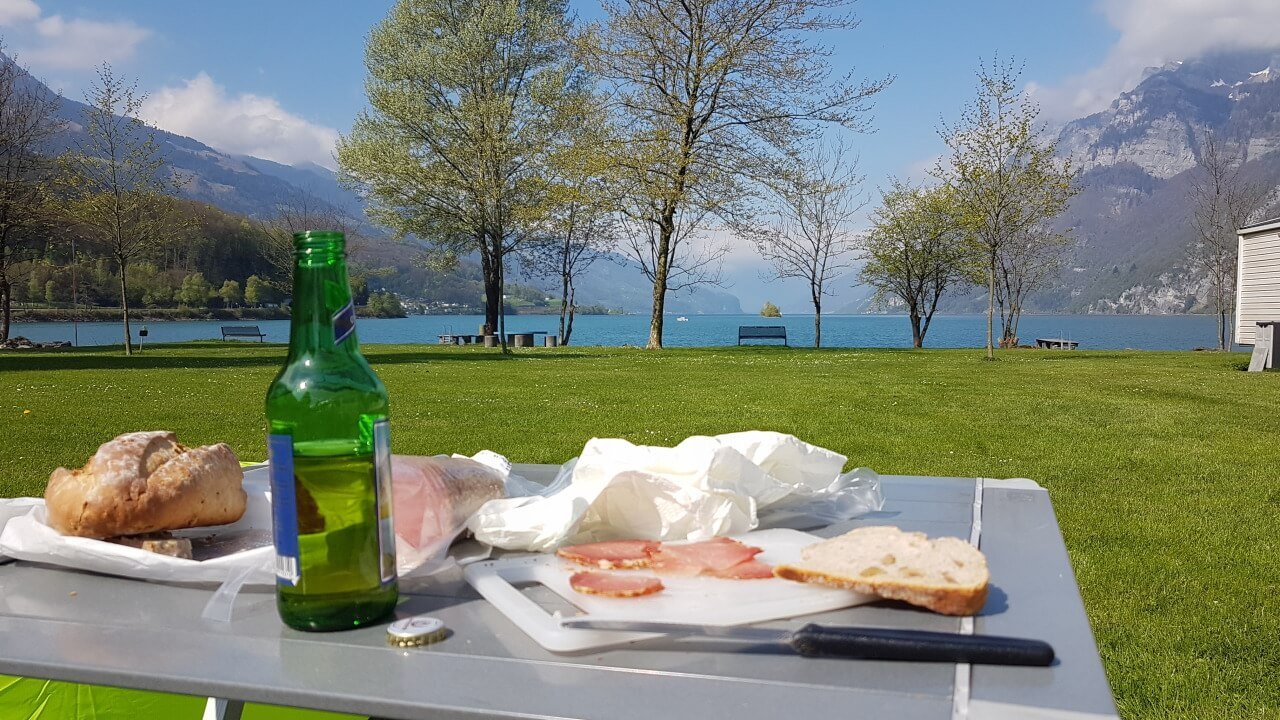
\includegraphics[width=0.4\textwidth, height=5cm, keepaspectratio]{../Bilder/Walensee/7.jpg}
    \caption{Picknick am Walensee}
  \end{centering}
\end{wrapfigure} 

\begin{figure}[b]
\centering
      %\subfloat[CAPTION]{BILDERCODE}\qquad
   \subfloat{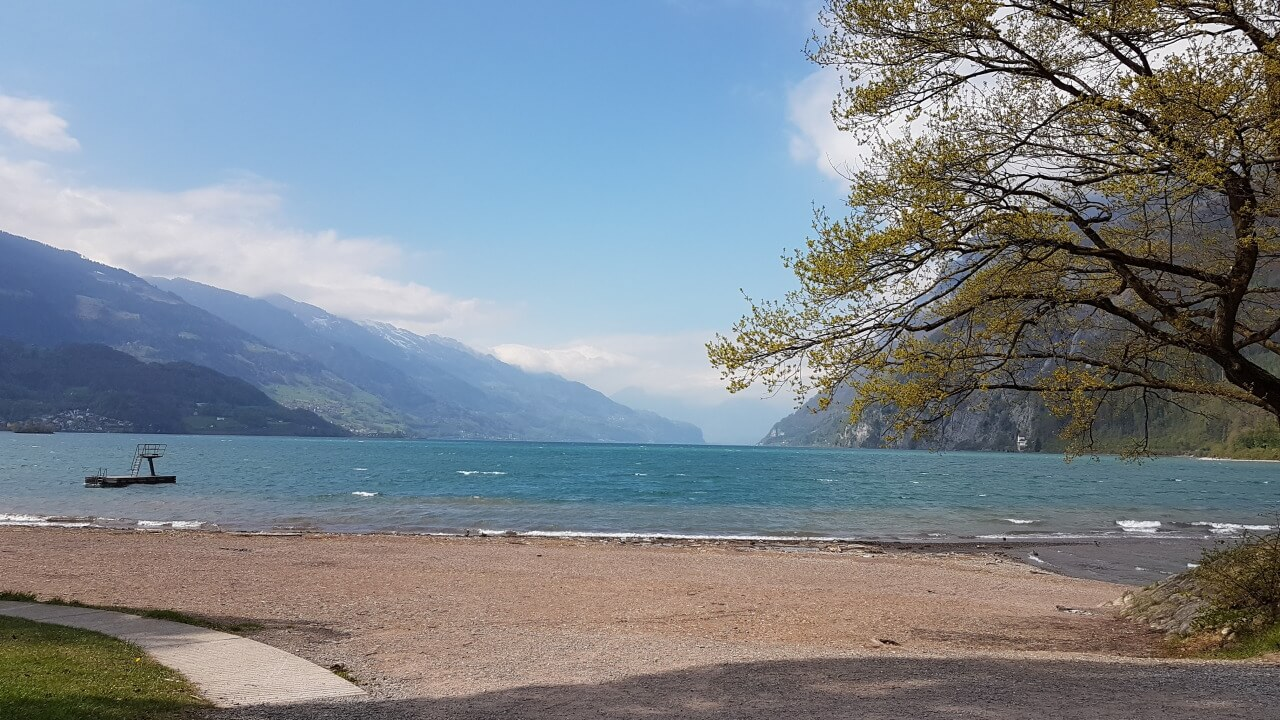
\includegraphics [width=0.3\textwidth]{../Bilder/Walensee/9.jpg}}\quad
   \subfloat{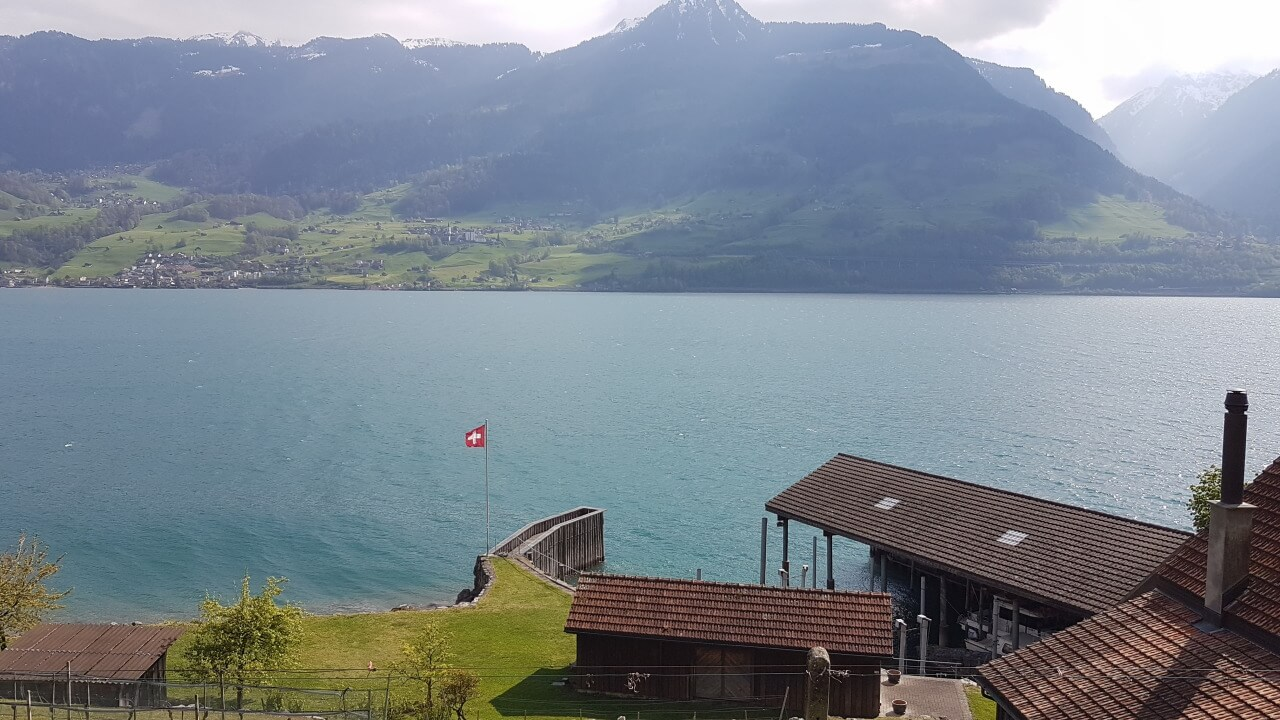
\includegraphics [width=0.3\textwidth]{../Bilder/Walensee/22.jpg}}\quad
   \subfloat{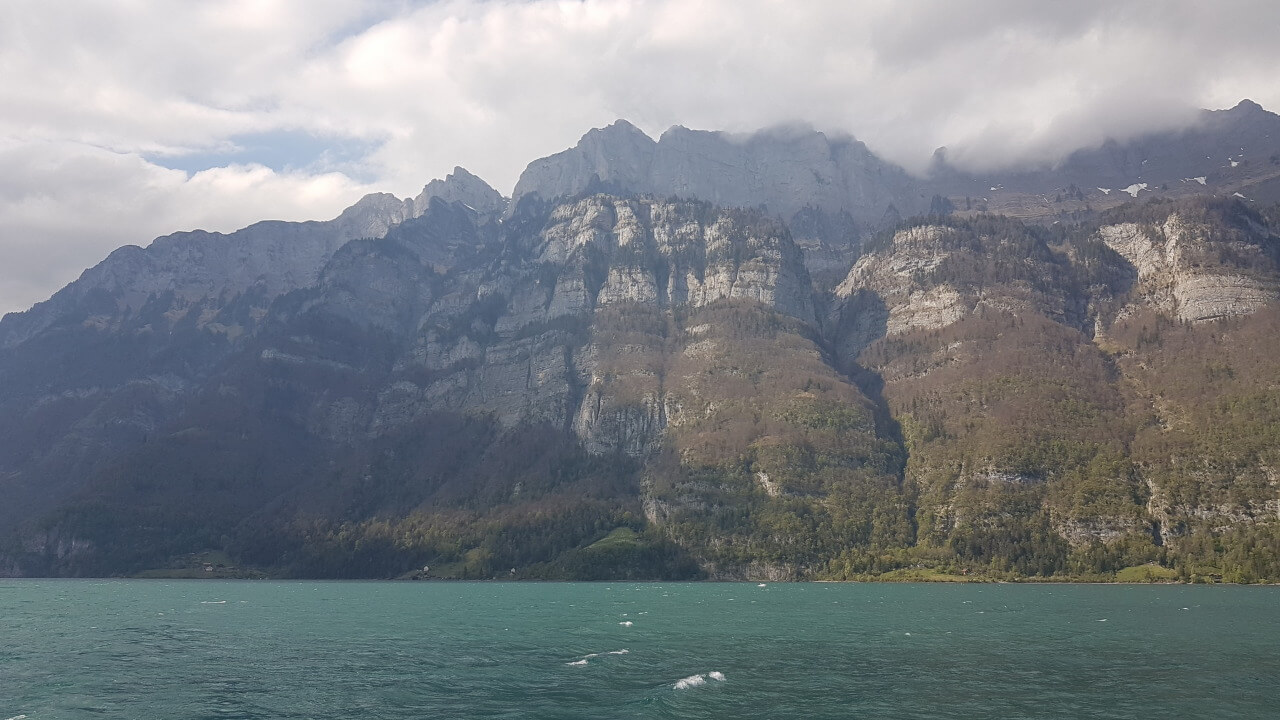
\includegraphics [width=0.3\textwidth]{../Bilder/Walensee/24.jpg}}\quad
   \caption[Wanderung am Walensee]{Wanderung am Walensee}
\end{figure}

Die Wetterprognosen und die Staulänge vor dem Gotthard motivierten für ein frühes Aufbrechen.
Das alljährliche vor dem Gotthardtunnel stehen hatte sich schon auf rekordverdächtige 14 Kilometer hoch gestanden was übersetzt hiess, dass das Wetter im Norden eher bescheiden sein wird.
Doch der Karfreitag versprach aus der Reihe zu tanzen.
Wolkenloser Himmel begrüsste uns und so machten wir uns kurz nach sieben bepackt mit Velos und dem nötigsten auf den Weg nach Nussbaumen, dem Heim unseres Busses. 
Nach dem Umladen der sieben Sachen und einem kurzen Halt um die Autobahn-Vignette zu kaufen sowie Treibstoff zu tanken ging es Richtung Zürich.
Das Wetter war bei der Abfahrt in Luzern um einiges besser als im Flachland.
Glücklicherweise verkehrte sich der Effekt wieder als wir wiederum Richtung Alpen fuhren.
Kurz nach dem Zürichsee zeigte sich das Wetter wieder von der besten Seite.
Die vielen Tafeln, welche vorschlugen den San Bernadino als Alternative zu benutzen zeigten noch keine Wirkung
und so konnten wir ohne Stau bis fast an den Walensee fahren.
Kurz nach Weesen hatten sich mehrere Fahrzeuge zur Kaltverformung zusammengefunden, wir hatten jedoch Glück und standen da maximal 10 Minuten.
Kurz darauf befanden wir uns auf der Ausfahrt Walenstadt.
Die Saison startete just heute für den Campingplatz See Camping.
Zusätzlich machten die miesen Wetterprognosen dem erwarteten Andrang einen Strich durch die Rechnung.
Die Auswahl der Stellplätze machte die Qual der Wahl nicht einfacher.
Direkt am See genossen wir so einen Imbiss bei schönstem Sonnenschein.

Noch heute, um das gute Wetter zu nutzen, sollte es auf grosse Wanderung gehen.
Dem Ufer des Walensee entlang nach Quinten oder Aue.
Der Walensee hat jedoch ziemlich steile Ufer, somit waren wir gezwungen einige Höhenmeter in Kauf zu nehmen um dem Ufer zu folgen.
Nach einem netten Schwatz mit einer Eingeborenen ging die Wanderung 500m über dem Walensee weiter.
Die einzige Möglichkeit sich den Rückweg per pedes zu ersparen bot das Kursschiff, welches
heute auch wieder den Betrieb aufnahm.
Dieses galt es unter keinen Umständen zu verpassen.
Unterwegs bemerkten wir, dass wir dank gutem Vorankommen Chancen haben das frühere Schiff zu erreichen und so vor dem Essen noch Duschen zu können.
Nach der kurzen Fahrt über den Walensee kamen wir an der schönen Uferpromenade in  Walenstadt an, welche sich wegen dem aufkommenden Wind schon massiv entvölkert hat.
Nach einem Apéro marschierten wir zurück zum Camping um nach einer Dusche die Fahrräder zu
satteln um uns einen feinen Fisch im Restaurant Seehof zu gönnen.
Nach der Rückkehr zum Bus schalteten wir die Standheizung in den Modus "`Sauna"'.
Dementsprechend unruhig war die erste Nacht des Jahres 2017 im Bus.


\subsection{15.04.2017 Fashion Outlet und Bündner Herrschaft}

\begin{wrapfigure}{L}{0.45\textwidth} 
  \begin{centering}
    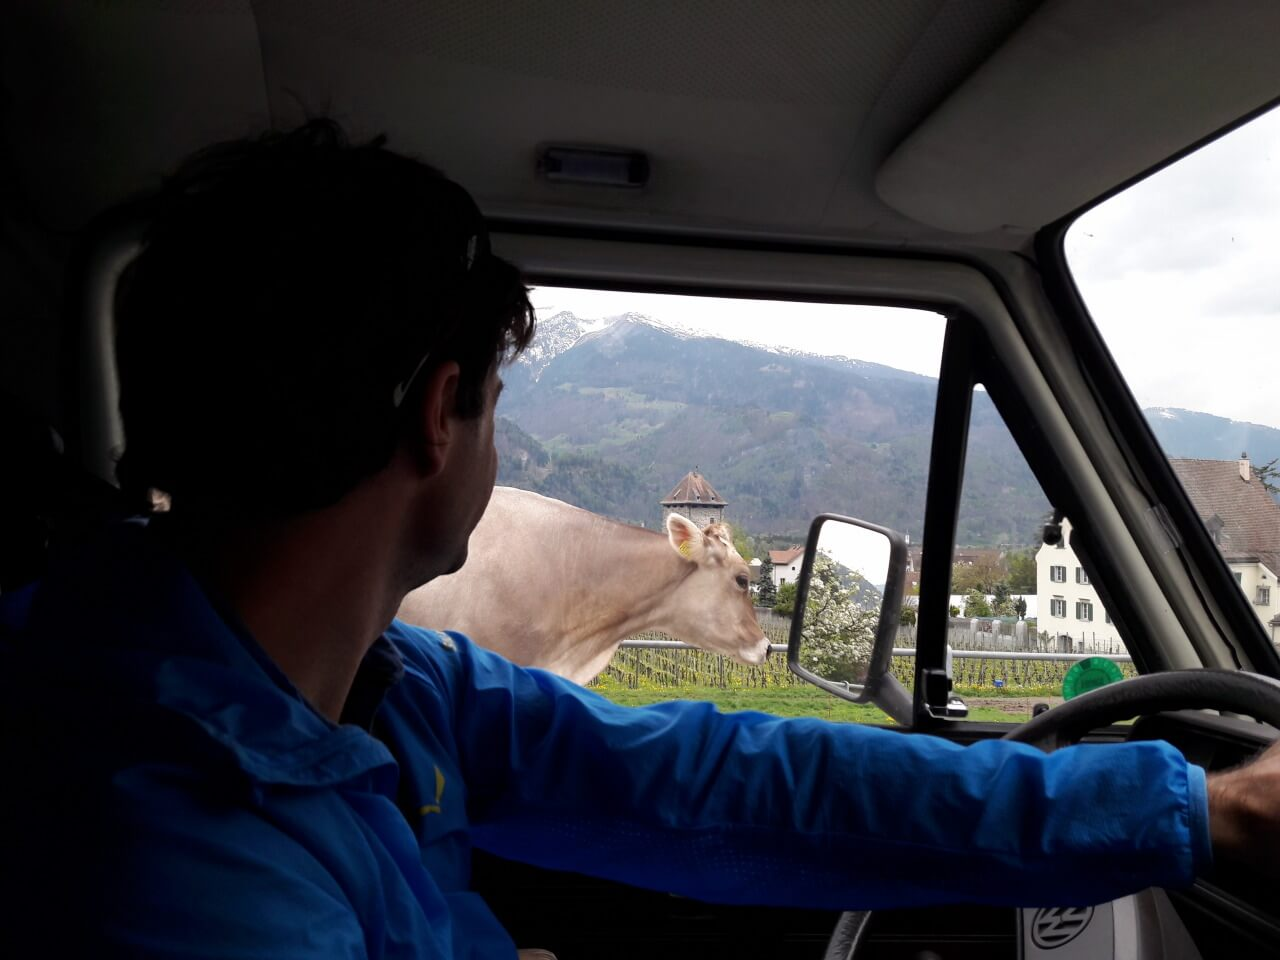
\includegraphics[width=0.4\textwidth, height=5cm, keepaspectratio]{../Bilder/Walensee/28.jpg}
    \caption{Kuh macht Ausflug}
  \end{centering}
\end{wrapfigure}

Nach einer eher unruhigen Nacht blinzelte schon früh die Sonne durch die Vorhänge was eigentlich so gar nicht vorgesehen war.
Der Wetterbericht war eher negativ und so beschlossen wir das  Fashion Outlet in Landquart unsicher zu machen.
Der Bus wurde nach dem Frühstück fahrbereit gemacht und kurz darauf befanden wir uns auf der Fahrt Richtung Chur.
Der Weg wurde genutzt um unsere weiteren kulinarischen Pläne in die Tat umzusetzen.
Wie meistens üblich wurden wir nach Bekanntgabe des Reiseziels mit sehr guten Tipps aus Dättwil überschüttet, welche Restaurants in der Gegend einen Besuch wert sind.
Aus diesem Grund sollte am Abend Murg angesteuert werden. 
Für die Eskalation im Fashion Outlet sorgte dann eher der untypische Teil eines Paares.
Ich tauchte schlussendlich schleppend wieder beim Bus auf und präsentierte Stolz meinen Fang.
Pfannenset, Zubehör und Bratpfannen haben es mir angetan.
Böse Zungen behaupten das Liege in der Familie¿
Der Himmel zog sich immer mehr zu und trotzdem wollten wir es nicht missen einen Blick auf die wunderschönen Dörfer in der Bündner Herrschaft zu werfen.
So durchquerten wir Malans, Jenins, Maienfeld und Fläsch und träumten von wärmeren Wetter und langen Abenden in den Torkel und Reben der Gegend. 
Dank dem sehr gut ausgebauten ÖV-Netz beschlossen wir den Bus für das Nachtessen stehen zu lassen und mit dem Bus nach Murg zu fahren.
Da wir noch eher früh dran waren konnten wir noch kurz das zum Restaurant gehörendem Lodge Hotel besuchen.
Nach einem Apéro hatten gewisse Teile der Crew von Jack schon wunderbar eines am Helm.
Das echt sehenswerte Restaurant versorgte uns mit wunderbaren Köstlichkeiten und der gute Wein tat den Rest  um den Abend zu einem Erfolg werden zu lassen.
Die Heimfahrt verging dann dank promillebedingter Betäubung wie im Flug.
Etwas muss jedoch noch erwähnt werden: Ich wusste gar nicht, dass am Bahnhof in Murg auch Dampfschiffe fahren.
Das Nebelhorn war auf jeden Fall gut zu hören.

\begin{figure}[H]
    \centering
    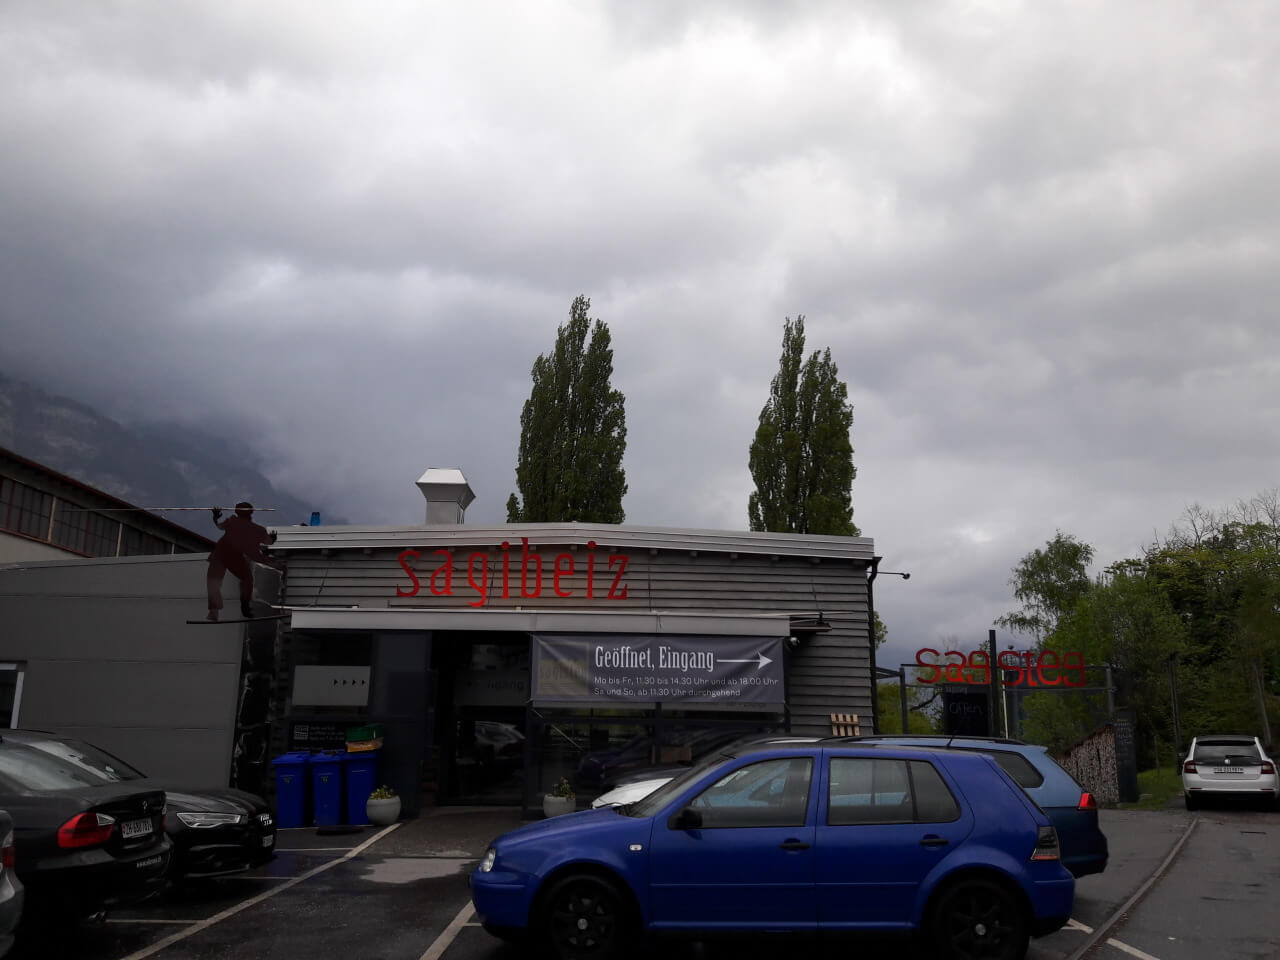
\includegraphics[width=\textwidth]{../Bilder/Walensee/31.jpg}
    \caption{Sagibeiz in Murg}
    \label{img:Sagibeiz}
\end{figure}

\subsection{16.04.2017 Bad Ragaz} 
Das gleichmässige Geräusch versprach nichts Gutes.
Es regnete und so sollte es denn ganzen Tag auch weitergehen.
Schon das Frühstück im Bus war eine Herausforderung und so kam bald einmal die Frage auf ob wir heute abfahren sollten oder noch eine Nacht ¿ausharren¿ sollten.
Die sprichwörtliche Bequemlichkeit entschied dann für uns und wir machten es uns im Bus gemütlich und planten den Besuch in der Tamina Therme in Bad-Ragaz.
Wenn schon Nass dann wenigstens 36.5°.
Tatsächlich hatte das Wetter kein Erbarmen und es regnete ununterbrochen weiter.
Nach einem Imbiss in der Bäckerei kamen wir durchnässt bei der Therme an.
Die nächsten 2 Stunden hiess es tüchtig aufwärmen und das sprudelnde Wasser geniessen, bevor uns ein weiteres Mal das eiskalte Wetter begrüsste.
Der Spaziergang vom Bahnhof Walenstadt zum Campingplatz war dieses Mal besonders lang. 
Alles durchnässte wurde behelfsmässig im Bus verteilt, so dass die Standheizung ihren Dienst tun konnte.
Das machte sie auch prompt und schon bald hatten wir eine Art künstliche Tropfsteinhöhle im Bus.
Erinnerungen an den Ausflug nach Ägeri wurden wach.
Das warme Wasser von Bad-Ragaz sowie das schlechte Wetter machten die Entscheidung leicht nicht mehr für das Abendessen auszugehen.
Somit war heute Ravioli Abend, was nicht gerade für Begeisterungsstürme seitens Chantal sorgte.
Die mitgebrachten Serien auf dem Laptop hatten ein leichtes Spiel uns in den Schlaf zu begleiten.

\subsection{17.04.2017 Zusammenpacken und Rückfahrt}
Glücklicherweise hatten wir eine Regenstopp der dazu genutzt werden konnte unsere Siebensachen einzupacken und uns auf den Weg Richtung Raststätte Glarnerland zu machen.
Die Churfirsten welche uns am Freitag noch frühlingshaft begrüssten, waren bei der Abfahrt wieder bis weit nach unten mit einer feinen Schneeschicht überzogen.

Die Region Walensee, wir werden sie garantiert ein weitere Mal besuchen...

\begin{figure}[H]
    \centering
    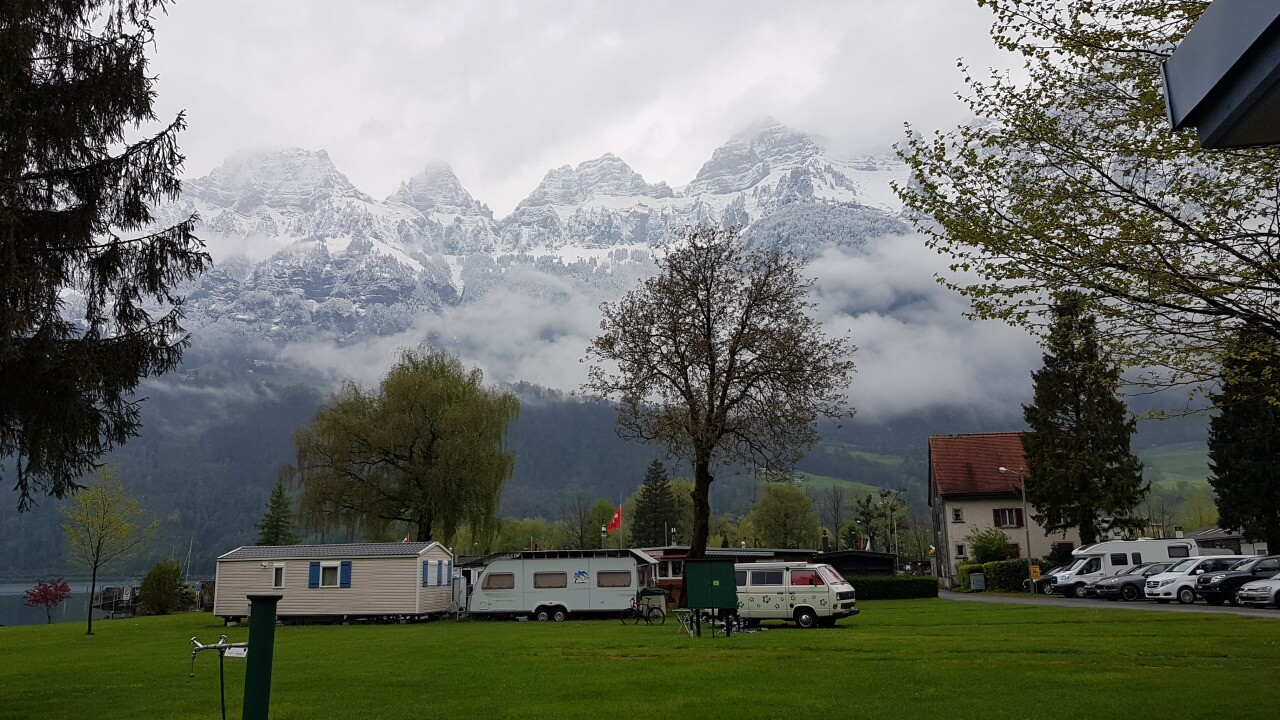
\includegraphics[width=\textwidth]{../Bilder/Walensee/35.jpg}
    \caption{Wieder verschneite Churfirsten}
    \label{img:Churfirsten}
\end{figure}
